\chapter{Digital pathology}
\label{chap:backdp}

\begin{overview}{Overview}
  The goal of this chapter is to provide digital pathology background  and keys to understand our contributions. We will focus our attention on topics relevant to this thesis. 
  
  Section \ref{sec:backdp:whatisdp} introduces and defines medical terms such as \textit{pathology}, defines \acrfirstit{dp} and introduces the notion of \acrfirstit{wsi}. Section \ref{sec:backdp:wsi} presents the journey of a sample from the body to the \acrshort{wsi}, introducing the different sources of variability introduced by the whole conversion process. 
\end{overview}

% analogintelligence.com image dp illustration

\section{What is digital pathology?}
\label{sec:backdp:whatisdp}

Nowadays, medicine and healthcare rely heavily on analysis of human body samples to study and diagnose diseases. The branch of medicine focusing on this analysis is called \textit{pathology} which includes histology-based pathology (\aka histopathology) and cytology-based pathology (\aka cytopathology). Both of these sub-branches involve the study of microscope glass slides containing samples (see Figure \ref{fig:backdp:glassslides}). In the case of histology, these samples are tissue sections cut from a bodily specimen. Cytology, on the other hand, is concerned with samples of free cells or tissue fragments which can be extracted by different techniques. 

\begin{figure}
  \centering
  \subfloat[Glass slide]{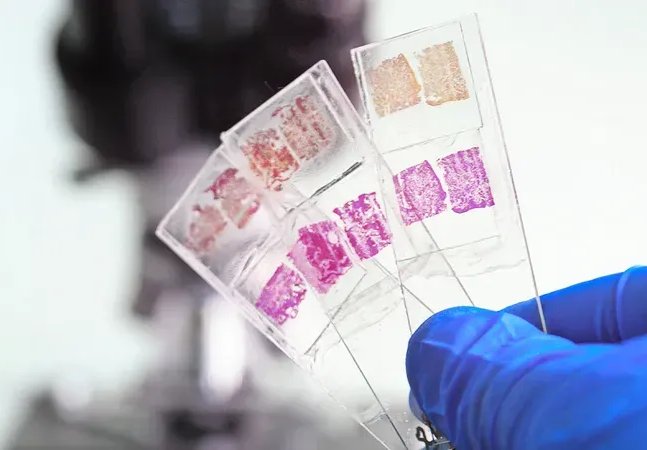
\includegraphics[scale=0.35]{backdp/microscope-slide.png}}\quad
  \subfloat[Whole-slide image]{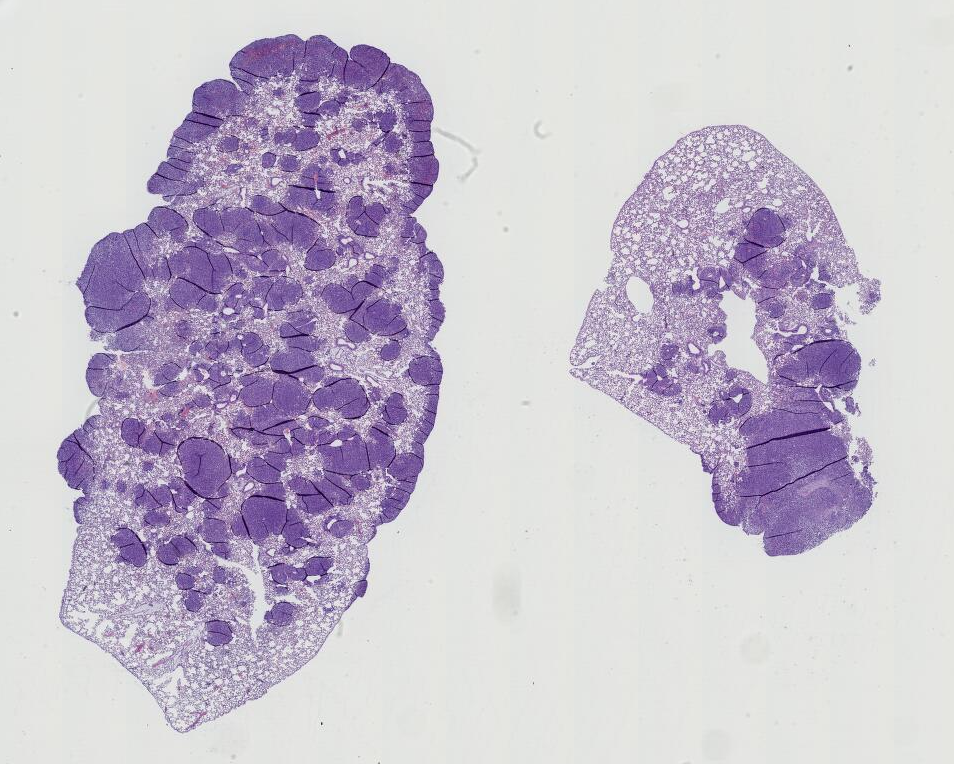
\includegraphics[scale=0.22]{backdp/wsi.png}}
  \caption{Microscope slides with tissue samples (images from \parencite{img:glassslides} and \TODO{reference demo cytomine}).}
  \label{fig:backdp:glassslides}
\end{figure}

The trend of digitalization affecting our societies also impacts pathology as, using dedicated scanners, these glass slides can now be digitized into large image files called \acrfirstit{wsi}. In this context, \acrfirstit{dp} can be defined as ``\textit{the acquisition, management, sharing and interpretation of pathology information — including slides and data — in a digital environment}'' \parencite{doolan2019whatisdp}. Working with \acrshort{wsi} instead of physical slides has several advantages and drawbacks (see Table 1 in \parencite{jahn2020digital} for a thorough list). Aside from easier sharing and storing of slides, digitization also opens the way for automated analysis sofware to automatically extract relevant information. Such software have the potential to relieve pathologists from time-consuming tasks allowing them to focus on challenging cases and research therefore reducing healthcare cost and improving diagnosis quality. According to the 2020 report on cancer from \acrfirstit{who} \parencite{world2020report}, the ratio of pathologist per inhabitant was approximately 1 per 15000 in high income countries but dramatically dropping to 1 er 1 million or less many low income countries. AI-assisted pathology therefore holds even greater promises for coverage and quality of healthcare in these countries where pathologists are rare.

Interestingly, although digitization technologies are quite mature, adoption of \acrlong{dp} in healthcare facilities is not simple. Many still heavily rely on glass slides for day-to-day operations. Indeed, the transformation requires significant investments (both in time and money) and careful planning to carry it out successfully which is not always comptabile with the workload of pathology services. Experienced pathologists are sometimes reluctant to change and lack confidence in modern tools for slide visualization and analysis. Moreover, some tasks cannot be performed easily on \acrlong{wsi}s but can on a glass slide (\eg exploring the depth of a sample in cytology by changing the focal plane). 

As far as automated analysis is concerned, it remains quite a challenge. Whole-slide images typically contain several gigapixels and cannot be loaded entirely in a typical computer memory at full resolution. Moreover, for most tasks, the image content is complex and classical computer vision methods would often fail to distinguish structures of interest. This complexity is due in particular to the presence of artifacts \parencite{taqi2018review} appearing during the conversion process of a bodily specimen to an image (see Section \ref{sec:backdp:wsi}). The ability of learning techniques to train models that capture complex relationships in data makes machine learning an ideal candidate to tackle \acrlong{dp} tasks. However, data scarcity is a prevalent issue in the field as quality data, especially annotated, can be difficult to obtain for various reasons: privacy concerns, time-consuming and expensive nature of the annotation process, \etc.     

Overall, digital pathology holds great promises but presents significant and interesting challenges on several fronts. This thesis focuses on the \acrshort{ml}-based automated analysis aspects of digital pathology and studies how to tackle data scarcity.

\section{A journey from the body to the computer}
\label{sec:backdp:wsi}

Turning a bodily specimen into \acrlong{wsi}s is a long and complex multi-step process typically involving the work of several highly-specialized technicians. Some steps can nowadays be automated but the chain remains mostly manual. In this section, we describe the different steps of this procedure (see \parencite{mccann2014automated} for an alternate presentation with illustrations). For the sake of brevity, this description focuses on histology with a tissue section prepared for brightfield microscopy and scanning, brightfield being one of the most common modality used in histo- and cytopathology. Sample preparation can differ more or less dependending on the nature of the sample (\eg histology, cytology, hematology) or target imaging technique (\eg brightfield, fluoresence, multispectral) but it is out of the scope this thesis to discuss these differences. 

During the description, we will discuss some of the possible visual and/or physical alterations of the sample resulting from a specific preparation step. The presence of these alterations, or artifacts, is one of the reason why processing \acrshort{wsi} manually or automatically can be challenging. Indeed, these alterations can at worst prevent any meaningful analysis by hiding, destroying or changing the appearance of the structures of interest. Our presentation of alterations and artifacts will not be exhaustive. A more thourough list of pre-scan artifacts with illustrations can be found in \parencite{taqi2018review}. 

\subsection{Samples collection, fixation, cutting and dehydratation}

Whereas we focus mostly on histo- and cyto-pathology in this thesis, a pathology service typically deals with more than these two modalities. The specimens they receive for analysis range from small (commonly referred to as \textit{biopsies}) to very large (whole organ or body). Whole bodies are usually destined for autopsies which might themselves generate biopsies. Smaller speciemens (organs, biopsies) must be fixated before going through the next steps. 

The goal of fixation is to put a stop to the natural decay of the specimen and increase its structural stability \parencite{rolls2012process}. This can be achieved, for instance, by immersing the specimen in a formaldehyde bath (\ie the fixative solution) for period of time depending on its size (\ie few hours to a whole day). 

When the specimen has been fixated, it is then placed into a standardized container called a \textit{cassette} (see Figure \ref{fig:backdp:cassette}). If the sample is too large for the cassette, a volume of interest is cut from the specimen. Depending on the later examination, the orientation of the cut can be crucial to exhibit relevant tissue structures of the specimen. In the remaininder, we will call a \textit{sample} the content of this cassette.

For a proper analysis, the cellular morphology of the sample must be preserved. This is most commonly achieved by infiltrating the tissue with paraffin wax. Infiltration however does not work on a raw fixated tissue because paraffin is hydrophobic. Therefore, one must first perform \textit{dehydratation}, that is, to replace water naturally present in the sample with a product miscible with parrafin. This is done by first plunging the sample into a succession of alcoholic solutions baths. Although this process achieve dehydratation, alcohol does not mix with paraffin neither. Therefore, the sample is then plunged into one or more xylene-based solutions baths, xylene being miscible with both alcohol and paraffin. The sample, infiltrated with xylene, is finally plunged in a paraffin bath under vacuum \TODO{how does it work the vaccum stuff???}. The dehydratation process takes few hours and is often automated using dedicated machines.  

Artifacts can appear as early as at extraction of the specimen and even before. Each of the specimen and sample processing steps presented in this section can also introduce artifacts. Tissue can be damaged at specimen extraction site by the use of medical tools or treatment. Bad fixation can lead to decaying tissue (\ie autolysis) and structural degradation (\eg tissue shrinkage). Improper cutting can also cause tissue damage like tearing, squeezing and burning. Dehydratation has also its own set of possible artifacts. Improper dehydratation can leave some parts of the sample with remaining water, alcholol or xylene which. Tissues can also be exposed to the different solutions for an excessive duration. These processing errors can for instance cause tearing, shrinkage, interference with the staining process (see Section \ref{ssec:backdp:staining}) and affect the structural properties of the tissue (\eg the tissue becomes brittle). Automation obviously reduces the risk of mistakes and artifacts.

\TODO{big figure illustrating ``all'' possible artifactsand variations}
\TODO{illustrate process}

% \begin{figure}
%   \centering
%   \subfloat[This is an example of well-fixed tissue showing good nuclear and cytoplasmic morphology with minimal shrinkage showing clearly defined basement membranes and cell margins.]{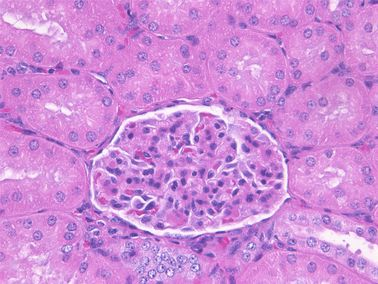
\includegraphics[scale=1.0]{backdp/fixationgood.png}\label{fig:backdp:goodfixation}}\quad
  
%   \subfloat[This is an example of poorly-fixed tissue showing inferior nuclear and cytoplasmic morphology with excessive shrinkage and poorly defined cell margins.]{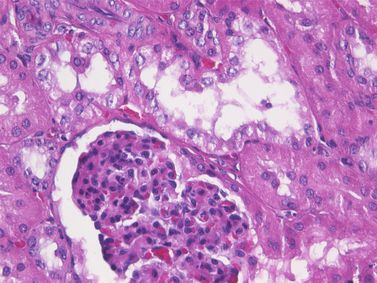
\includegraphics[scale=1.0]{backdp/fixationbad.jpg}\label{fig:backdp:badfixation}}
    
%   \caption{Examples of good and bad fixations (images and sub-captions from \parencite{rolls2012process}).}
%   \label{fig:backdp:fixation}
% \end{figure}

\begin{figure}
  \centering
  \subfloat[Cassette with fixated samples (image \\ from \parencite{stidworthy2011getting})]{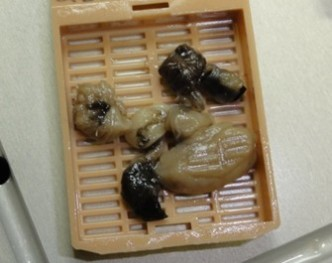
\includegraphics[scale=0.75]{backdp/cassette.jpg}\label{fig:backdp:cassette}}\quad
  \subfloat[Cassette with parrafin-embedded \\ samples (image from \parencite{img:cassetteparrafin})]{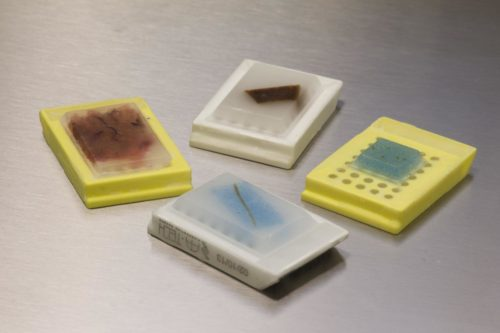
\includegraphics[scale=0.42]{backdp/cassette-parrafin.jpg}\label{fig:backdp:cassette-parrafin}}
  \caption{Tissue cassettes.}
\end{figure}

\subsection{Embedding, microtomy and glass-slide application}
\label{ssec:backdp:embedding}

At this point, the sample in the cassette has been infiltrated with paraffin. The next step consists in embedding the infiltrated sample in a block of paraffin to allow easier cutting. The sample is placed in a small container attached to the back of the cassette. This container will serve as a mold for casting the block of parrafin (see Figure \ref{fig:backdp:cassette-parrafin}). When the block has solidified, the sample can now be cut into thin slices to be applied on the glass slides. Cutting is performed with a dedicated tool called a \textit{microtome} (see Figure \TODO{illus microtome}). Operated by a technician, the microtome allows slices to be cut to an extremely small and precise thickness of around 3 or 4 $\mu m$. The cutted slices are then floated onto a water bath which helps mouting them on glass-slides. 

These steps should be performed carefully not to introduce artifacts. For instance, a warm parrafin block or a dull microtome blade can cause compression artifacts (\ie tissue displacement causing material accumulation). Another possible source of artifact is contamination of the water bath with previous samples, hair, dust which can in turn contaminate the floating slices.   

\subsection{Staining}
\label{ssec:backdp:staining}
At this point, mounted tissue slices are almost completely transparent which would prevent any meaningful analysis. They must therefore be stained to highlight structures of interest. Similarly as for dehydratation, this process consists in bathing the slide into a succession of stainning solutions. The nature of these solutions will depend on the content that should be highlighted for the future analysis. The most common and standard staining in histology is called \acrfirstit{heeo}. Hematoxylin stains nucleic acids in a deep blue-purple color (typically cell nuclei) and eosin nonspecifically stains proteins in a pink color (typically extracellular matrix and cytoplasm). An example of an \acrshort{heeo} slide is given in Figure \TODO{illus \acrshort{heeo}}. The \acrshort{heeo} stain, although most common, is not the only available. There exists many other staining techniques such as \acrfirstit{ihc} which exploits the binding nature of some antibodies with specific proteins. Markers can then be used to highlight the antibodies, hence the proteins of interest they have bound with. Example of an \acrshort{ihc}-stained slide is given in Figure \TODO{illu \acrshort{ihc}}. When the sample has been stained and cleaned from remaining excess of staining solutions, one must apply a cover slip on the sample in order to ensure that sample lies in one single plane as the focal plane of microscopes and scanners is usually quite narrow. The cover slip also protects the sample from external contamination and degradation. 

The choice of a staining and its clean application are crucial for an efficient analysis. The staining baths can become contaminated with samples, by-products resulting from chemical reactions (\eg precipitation or crystallization of chemical components resulting in the presence of pigments in the sample) or external objects (\eg hair, dust). The baths usually degrade over time and use which can cause variation in the staining intensities between earlier and later samples. The bath duration is important for proper staining and bathing samples for less or more time than recommanded can respectively cause under- or over-staining. Moreover, insufficient cleaning after staining can leave spots of stain on the slide. Improper application of the cover slip can for instance cause the presence of air bubbles. Nowadays, the staining process can be automated with dedicated machine reducing the variability of the process. 

\subsection{Scanning}
\label{ssec:backdp:scanning}

A glass slide coming out of the staining process described in Section \ref{ssec:backdp:staining} is ready to be analysed with an optical microscope but can also be digitized by a slide scanner (see Figure \TODO{illustrate a scanner}) into a \acrshort{wsi}. As briefly explained in Section \ref{sec:backdp:whatisdp}, the use of digital slide offers new ways to interact with a sample and opens the way for the use of new analysis tools.

Scanners are equipped with high-precision lenses and sensors allowing them to generate very high-resolution images required for a proper analysis. A scanner typically scans images at the standard $\times$20 or $\times$40 magnifications (\ie resulting samples appear 20 or 40 times larger than they actually are) which are often enough for routine analysis of \acrshort{heeo} or \acrshort{ihc} slides \parencite{zarella2019practical}. Higher magnification are also available with dedicated scanners if required for the analysis. Given the need for such a magnification and resolution, it is not possible to capture the whole slide in a single shot with currently available sensors. Therefore, scanners typically capture a sample step by step either tile by tile or in a in-line fashion (see Figure \TODO{tile-line-scanning.jpg} from \parencite{jahn2020digital}) and then assemble together the different parts using a stitching algorithm. Obviously, as a slide is scanned in several shots, the scanner must ensure that focus is correct for all the shots in order to avoid blur. Common focus strategies are for instance re-focusing every tile, or every $n^{\text{th}}$ tile. When it comes to the focus strategy, there is usually a trade-off between scanning time and focus precision: focusing every tile allows for ideal focus but takes time, whereas focusing every $n^{\text{th}}$ is faster but incurs a risk of incorrect focus and blur between the re-focusing steps. Thanks to different tricks, scanning time per slide nowadays ranges from 30 seconds to several minutes. These tricks include improved focus strategies and automatic tissue detection allowing to skip the empty parts of the slide during scanning. Most scanners also allow to load batches of few hundreds of slide at once therefore reducing the time spent interacting with the machine.

Scanning can also introduce artifacts including stiching problems (\ie misalignment between scanned tiles or lines), blur due to incorrect focus, tissue detection failure causing parts of the slide to be missing from the \acrshort{wsi}. The scanner should obviously remain as clean as possible to avoir external components to pollute the image (\eg dust, glass shards, hair, \etc). 

\section{Typical diagnosis tasks}
\label{sec:backdp:typicaldiagnosistasks}

When a slide has finally been prepared, pathologists take over and can start the analysis, whether on a computer screen or through the lenses of an optical microscope. One of the most frequent condition that has to be evaluated is malignancy of tumors but other diagnosis can also be performed on the basis of pathology slides. The indicators of malignancy can vary greatly from a disease to another and even from one type of cancer to another. The approach of the slide by the pathologist and the analysis can therefore vary accordingly. Some analysis can be qualitative but some diagnosis require grading the severity of the disease which is usually based on a quantitive evaluation of some indicators. 

Sometimes diagnosis require to evaluate tissues appearance, shape or localization at a macroscopic level\TODO{illustrate with images and examples}. For instance, localizing a malignant tumor in its support tissue can be important for guiding a future surgical operation \TODO{double check}. Measuring the size of a tumor (by measuring its surface on the slide) is useful for grading cancer. Evaluating whether a tumor still in-situ (\ie cancer cells have not spread from the location where they first formed) or proliferative is also paramount for determining a propre treatment as proliferation opens the possibility of metastases.  

Some analysis require to look at tissues at a more microscopic level. A single cell with a specific morphology in a slide\footnote{The extent of a tissue on a slide can be several orders of magnitude larger than the dimensions of the cells it contains.} can determine the malignant nature of a sample. A common, relatively simple yet time-consuming task is counting the number of mitosis (\ie cell division \TODO{figure}) in a tissue which is required for grading some cancer.

\section{Machine learning}
\label{sec:backdp:ml}

Digital pathology has opened the way for the application of \acrlong{ml} to automate analysis and diagnosis. Albeit promising, application of \acrlong{ml} remains challenging for various reasons. In this section, we discuss some of these challenges in Sections \ref{ssec:backdp:dataleakage} and \ref{ssec:backdp:datascarcity} then present some techniques that can be used, if not to overcome them, at least to alleviate them.

\subsection{Data leakage}
\label{ssec:backdp:dataleakage}

In Section \ref{ssec:backml:modelselinpractice}, we introduced the notion of data leakage that occurs when samples in different splits of a dataset are not independent from each other. Data leakage usually results in poor generalization performance when a \acrlong{ml} model is used in production. Obviously, this should be avoided at all cost especially when the prediction of this model impacts the patient diagnosis and treatment. It is worth noting that data leakage is considered an important obstacle for the application of \acrlong{ml} in biology and medicine in general, not only in \acrlong{dp} \parencite{ching2018opportunities}. 

In \acrlong{dp}, data leakage can occur in many, sometimes subtle, ways. Therefore, learning pipelines should be built carefully. One important potential source of data leakage is due to the fact that a whole-slide image does not only convey information about the tissue it contains but also about the slide preparation process (see Section \ref{sec:backdp:wsi}). For instance, staining solutions decay over time. Therefore, the staining intensity can reflect whether the sample has been dipped in a recently-changed or an heavily-used staining bath. When staining is performed manually, the intensity might also reflect the identity of the technician who performed the staining operation. Indeed, some technicians might dip slides for a little longer than others resulting in a stronger intensity. When a dataset is built by different laboratories, the origin of a slide can traceable due to differences in the slide preparation processes between the sites. 

These slide idiosyncracies are harmless as long as they are not correlated with the learning problem target. Whereas it might seem unlikely to happen, some simple though unfortunate choices can lead to correlation. For instance, supposing a problem of malignancy assessment, if one laboratory provides all the healthy samples and another all the malignant samples, there is significant risk that the learning algorithm would exploit the differences resulting from the preparation processes. This would obviously lead to poor generalization when the model will be applied to slide coming from another laboratory for instance. This could occur similarly if malignant and healthy slides are provided by the same laboratory but the former are prepared in the morning and the latter in the afternoon.

The slide preparation process is not the only culprit for data leakage. One other possible source occurs at the patient level. \parencite{bussola2021ai} \TODO{test score worse for patient wise splitting than for tile wise splitting in the article. That's unexpected.} have empirically studied patient-wise and random dataset splitting strategies. They have shown that overfitting and data leakage indeed occurs when splitting samples randomly. 

In general, it is difficult to completely prevent data leakage as one does not always have control over the whole \acrshort{wsi} generation process. However, good practices surely help reducing the problem to an acceptable minimum. A detailed list of guidelines and good practices to reduce the risk of data leakage can be found in \parencite{maree2017need}. This includes collecting data as representative as possible of the different variations that could naturally occur during the generation process. For model evaluation and selection, splitting the dataset into subsets should be performed considering the characteristics of the samples that could correlate with the target (\ie patient, laboratory, technician, staining, equipement, time of the day/week, \etc).

\subsection{Data scarcity}
\label{ssec:backdp:datascarcity}
% and imperfect annotations

As introduced in Section \ref{ssec:backml:sl}, \textit{data scarcity} refers to a context where data is lacking which usually hampers the performance of \acrlong{ml} methods, especially \acrlong{dl}. Data scarcity is often cited as one of the major challenges in \acrlong{dp} \parencite{tizhoosh2018artificial,litjens2017survey,robertson2018digital,komura2018machine}. A misconception would be to consider that data simply does not exist in a sufficient quantity. Indeed, hospitals and research institutes have accumulated a significant amount of data in different formats over the years (\eg imaging, text, \etc). What makes \acrlong{dp} but also the whole field of medical and biological image analysis a data scarce domain is a combination of factors preventing this data to be usable for \acrlong{ml} in a straightforward way.

More or less recent successes in the application of machine and \acrshort{dl} to natural images problems have been propelled by the existence of numerous large and exhaustively annotated datasets. For instance, the ImageNet classification dataset features 1000 fine-grained classes for 1.2 million images and has been a key element in my \acrlong{dl} innovations since AlexNet. Another example is \acrfirstit{coco} by Microsoft \parencite{lin2014microsoft}, a large-scale dataset for segmentation, detection and captioning (\TODO{present captioning in chapter 1}). It contains more than 200k images annotated with fine segmentation masks over objects from 91 distinct categories (\ie humans, furnitures, animals, \etc). It counts more than 800k unique annotated instances of these categories. Initially published by Google in 2016, the most recent iteration of Open Images Dataset \parencite{kuznetsova2020open} contains approximately 9.2 million images each annotated with one or more labels from 19.8k concepts for a total of 30 million image-level labels. \TODO{figure to provide examples of these dataset}. 

Those were only few examples of the plethora of datasets available in the natural image domain. In \acrlong{dp}, although the data scarcity situation is slowly improving, as the interest for \acrshort{ml}-based solutions has encouraged researchers and practitioners to increasingly share data and annotations, dataset size and versatility are still subpar compared to the natural image domain. In order to illustrate this point, we performed a search on the GrandChallenge website \parencite{grandchallange}, a popular plateform which runs \acrlong{ml} challenges related to biomedical images. We searched for \textit{histology} challenges published in 2021 and found eight results. All datasets are briefly described in Table \ref{tab:backdp:datascarcity-grandchallenge}. 

Depending on the target task, \acrshort{dp} datasets are either provided as a set of \acrlong{wsi}s or \acrfirstit{roi} extracted from \acrshort{wsi}s. 

\begin{table}
  \centering
  \small
  \begin{tabular}{|cc|cccccc|}
    \hline
    \multicolumn{2}{c}{Dataset} & \# \acrshort{wsi} & \# \acrshort{roi} & \acrshort{roi} size & AI-assisted & Number of target \\
    \hline
    \multirow{3}{*}{TIGER [1]} & wsitils &  & & & & yes & \\
    & wsirois & & & & & no & \\
    & wsibulk & & & & & no & \\
    CoNiC [2] & &  & & & & yes & \\
    MIDOG 2021 [3] & &  & & & & yes & \\
    BCNB [4] & &  & & & & no & \\
    WSSS4LUAD [5] & &  & & & & no & \\
    BCSS [6] & &  & & & & no & \\
    NuCLS [7] & &  & & & & yes & \\
    PAIP 2021 [8] & &  & & & & no & \\
    \hline
  \end{tabular}
  \caption{
  [1] \parencite{}, [2] \parencite{graham2021conic}, [3] \parencite{aubreville2021mitosis}, [4] \parencite{xu2021predicting}, [5] \parencite{han2021multilayer}, [6] \parencite{amgad2019structured}, [7] \parencite{amgad2021nucls}, [8] \parencite{}}
  \label{tab:backdp:datascarcity-grandchallenge}
\end{table}

% interest of the ML community
% many source but no annotations: cite few dataset sources
% variability, noise and uncertainty (disagreement between pathologists)
% class imbalance
% privacy

\subsection{Data dimensionality}
\label{ssec:backdp:datadimensionality} 

\TODO{talk about how such a complex specimen->slide process can cause variations from a lab to another}

\subsection{Data augmentation}


\subsection{Transfer learning}
\label{ssec:backdp:tl}

\parencite{van2019strategies}

\section{Visualization, analysis and benchmarking tools}

\subsection{Cytomine}

\subsection{Biaflows}

\subsection{Others}

\section{Digital pathology datasets}
\label{sec:backdp:dataset}


% origin, acknowledgements, subject, organ, staining, statistics


\subsection{Thyroid nodule fine-needle aspiration biopsy}



\subsection{Publicly available}